\section{Auswertung}

\subsection{Eichung des Elektromagneten}
Zu Beginn muss der verwendete Elektromagnet geeicht werden. Dazu wird die Magnetfeldstärke abhängig von der eingestellten Stromstärke vermessen. Aufgrund der Hysterese wird die Magnetfeldstärke
bei steigendem und bei fallendem Strom gemessen. Die Messwerte sind in Tabelle \ref{tab:B} und in Abbildung \ref{fig:plot} dargestellt.
\begin{table}
  \centering
  \caption{Messwerte der Magnetfeldstärke abhängig von der Stromstärke.}
  \label{tab:B}
  \begin{tabular}{S[table-format=2] S[table-format=3] S[table-format=3]}
    \toprule
    {$I$ / A} &  {$B$ / mT} & {$B$ / mT} \\
    {} & {(steigend)} & {(fallend)} \\
    \midrule
    0 &    4 &     5 \\
    1 &   71 &   74 \\
    2 &  129 &  131 \\
    3 &  195 &  179 \\
    4 &  253 &  240 \\
    5 &  307 &  308 \\
    6 &  368 &  370 \\
    7 &  428 &  420 \\
    9 &  556 &  555 \\
    8 &  488 &  472 \\
    10 & 614 &  609 \\
    11 & 661 &  668 \\
    12 & 723 &  730 \\
    13 & 777 &  779 \\
    14 & 830 &  841 \\
    15 & 872 &  888 \\
    16 & 948 &  923 \\
    17 & 972 &  972 \\
    \bottomrule
  \end{tabular}
\end{table}

Eine lineare Regression der Messwerte
\begin{equation}
  B(I) = aI + b
\end{equation}
ist ebenfalls in Abbildung \ref{fig:plot} dargestellt und ergibt die Parameter
\begin{align*}
  a &= \SI{57.9 \pm 0.4}{\frac{mT}{A}} \\
  b &= \SI{18 \pm 4}{mT}\,.
\end{align*}
Diese Funktion wird im Folgenden verwendet, um die Magnetfeldstärke bei den einzelnen Messreihen zu berechnen.

\begin{figure}
  \centering
  \includegraphics{plots/plot.pdf}
  \caption{Magnetfeldstärke abhängig von der Stromstärke.}
  \label{fig:plot}
\end{figure}

\subsection{Messung der Landé-Faktoren}
Zur Bestimmung der Landé-Faktoren wird die Verschiebung $\symup{\delta}$ der Wellenlänge in die entsprechende Energiedifferenz $\upD E$ umgerechnet:
\begin{align}
  |\upD E| &= \biggl|\frac{\partial E}{\partial\lambda}\biggr|\symup{\delta}\lambda \\
          &= \frac{\symup{ch}}{\lambda^2}\symup{\delta}\lambda \,.
  \label{eq:dE}
\end{align}
Der Landé-Faktor ergibt sich aus den Gleichungen \eqref{eq:dE_norm} und \eqref{eq:dE}:
\begin{align}
  g &= \frac{|\upD E|}{\mu_\text{B} B} \\
    &= \frac{\symup{ch}\cdot\symup{\delta}\lambda}{\lambda^2\mu_\text{B}B}\,.
\end{align}
Die Wellenlängenverschiebung $\symup{\delta}\lambda$ ergibt sich aus den Abständen der aufgenommenen Spektrallinien:
\begin{equation}
  \symup{\delta}\lambda = \frac{1}{2}\frac{\symup{\delta}s}{\upD s}\upD \lambda_\text{D}\,,
  \label{eq:versch}
\end{equation}
wobei $\upD s$ der Abstand zwischen den Spektrallinien ohne äußeres Magnetfeld, $\symup{\delta} s$ der Abstand zwischen den aufgespaltenen Linien
im Magnetfeld und $\upD\lambda_\text{D}$ das Dispersionsgebiet ist.
Das Dispersionsgebiet ergibt sich aus Formel % hier Referenz einfügen
und ist für die beiden betrachteten Linien in Tabelle \ref{tab:disp} dargestellt.
Zur Bestimmung der Abstände $\upD s$ und $\symup{\delta}s$ aus den Fotos wurden mit einem Grafikprogramm Linien durch die Intensitätsmaxima gezeichnet
und dann die Abstände zwischen den Linien in Pixeln bestimmt.

\begin{table}[h]
  \centering
  \caption{Wellenlängen und Dispersionsgebiet der untersuchten Linien.}
  \label{tab:disp}
  \begin{tabular}{c S[table-format=3.1] S[table-format=2.2]}
    \toprule
    Farbe & {$\lambda\:/\:\si{nm}$} & {$\upD\lambda_\text{D}\:/\:\si{pm}$} \\
    \midrule
    rot  & 643.8 & 48.91 \\
    blau & 480.0   & 26.95 \\
    \bottomrule
  \end{tabular}
\end{table}
%
\ \\
Zunächst wurden die Landé-Faktoren der roten Linie bestimmt. Bei der $\pi$-Linie zeigt sich, dass es keine Zeeman-Aufspaltung gibt, wie in Abbildung \ref{fig:r_pi} zu sehen ist. Dies deutet
darauf hin, dass der Landé-Faktor für die rote $\pi$-Linie 0 ist.
\begin{figure}
  \centering
  \begin{subfigure}{0.48\textwidth}
    \centering
    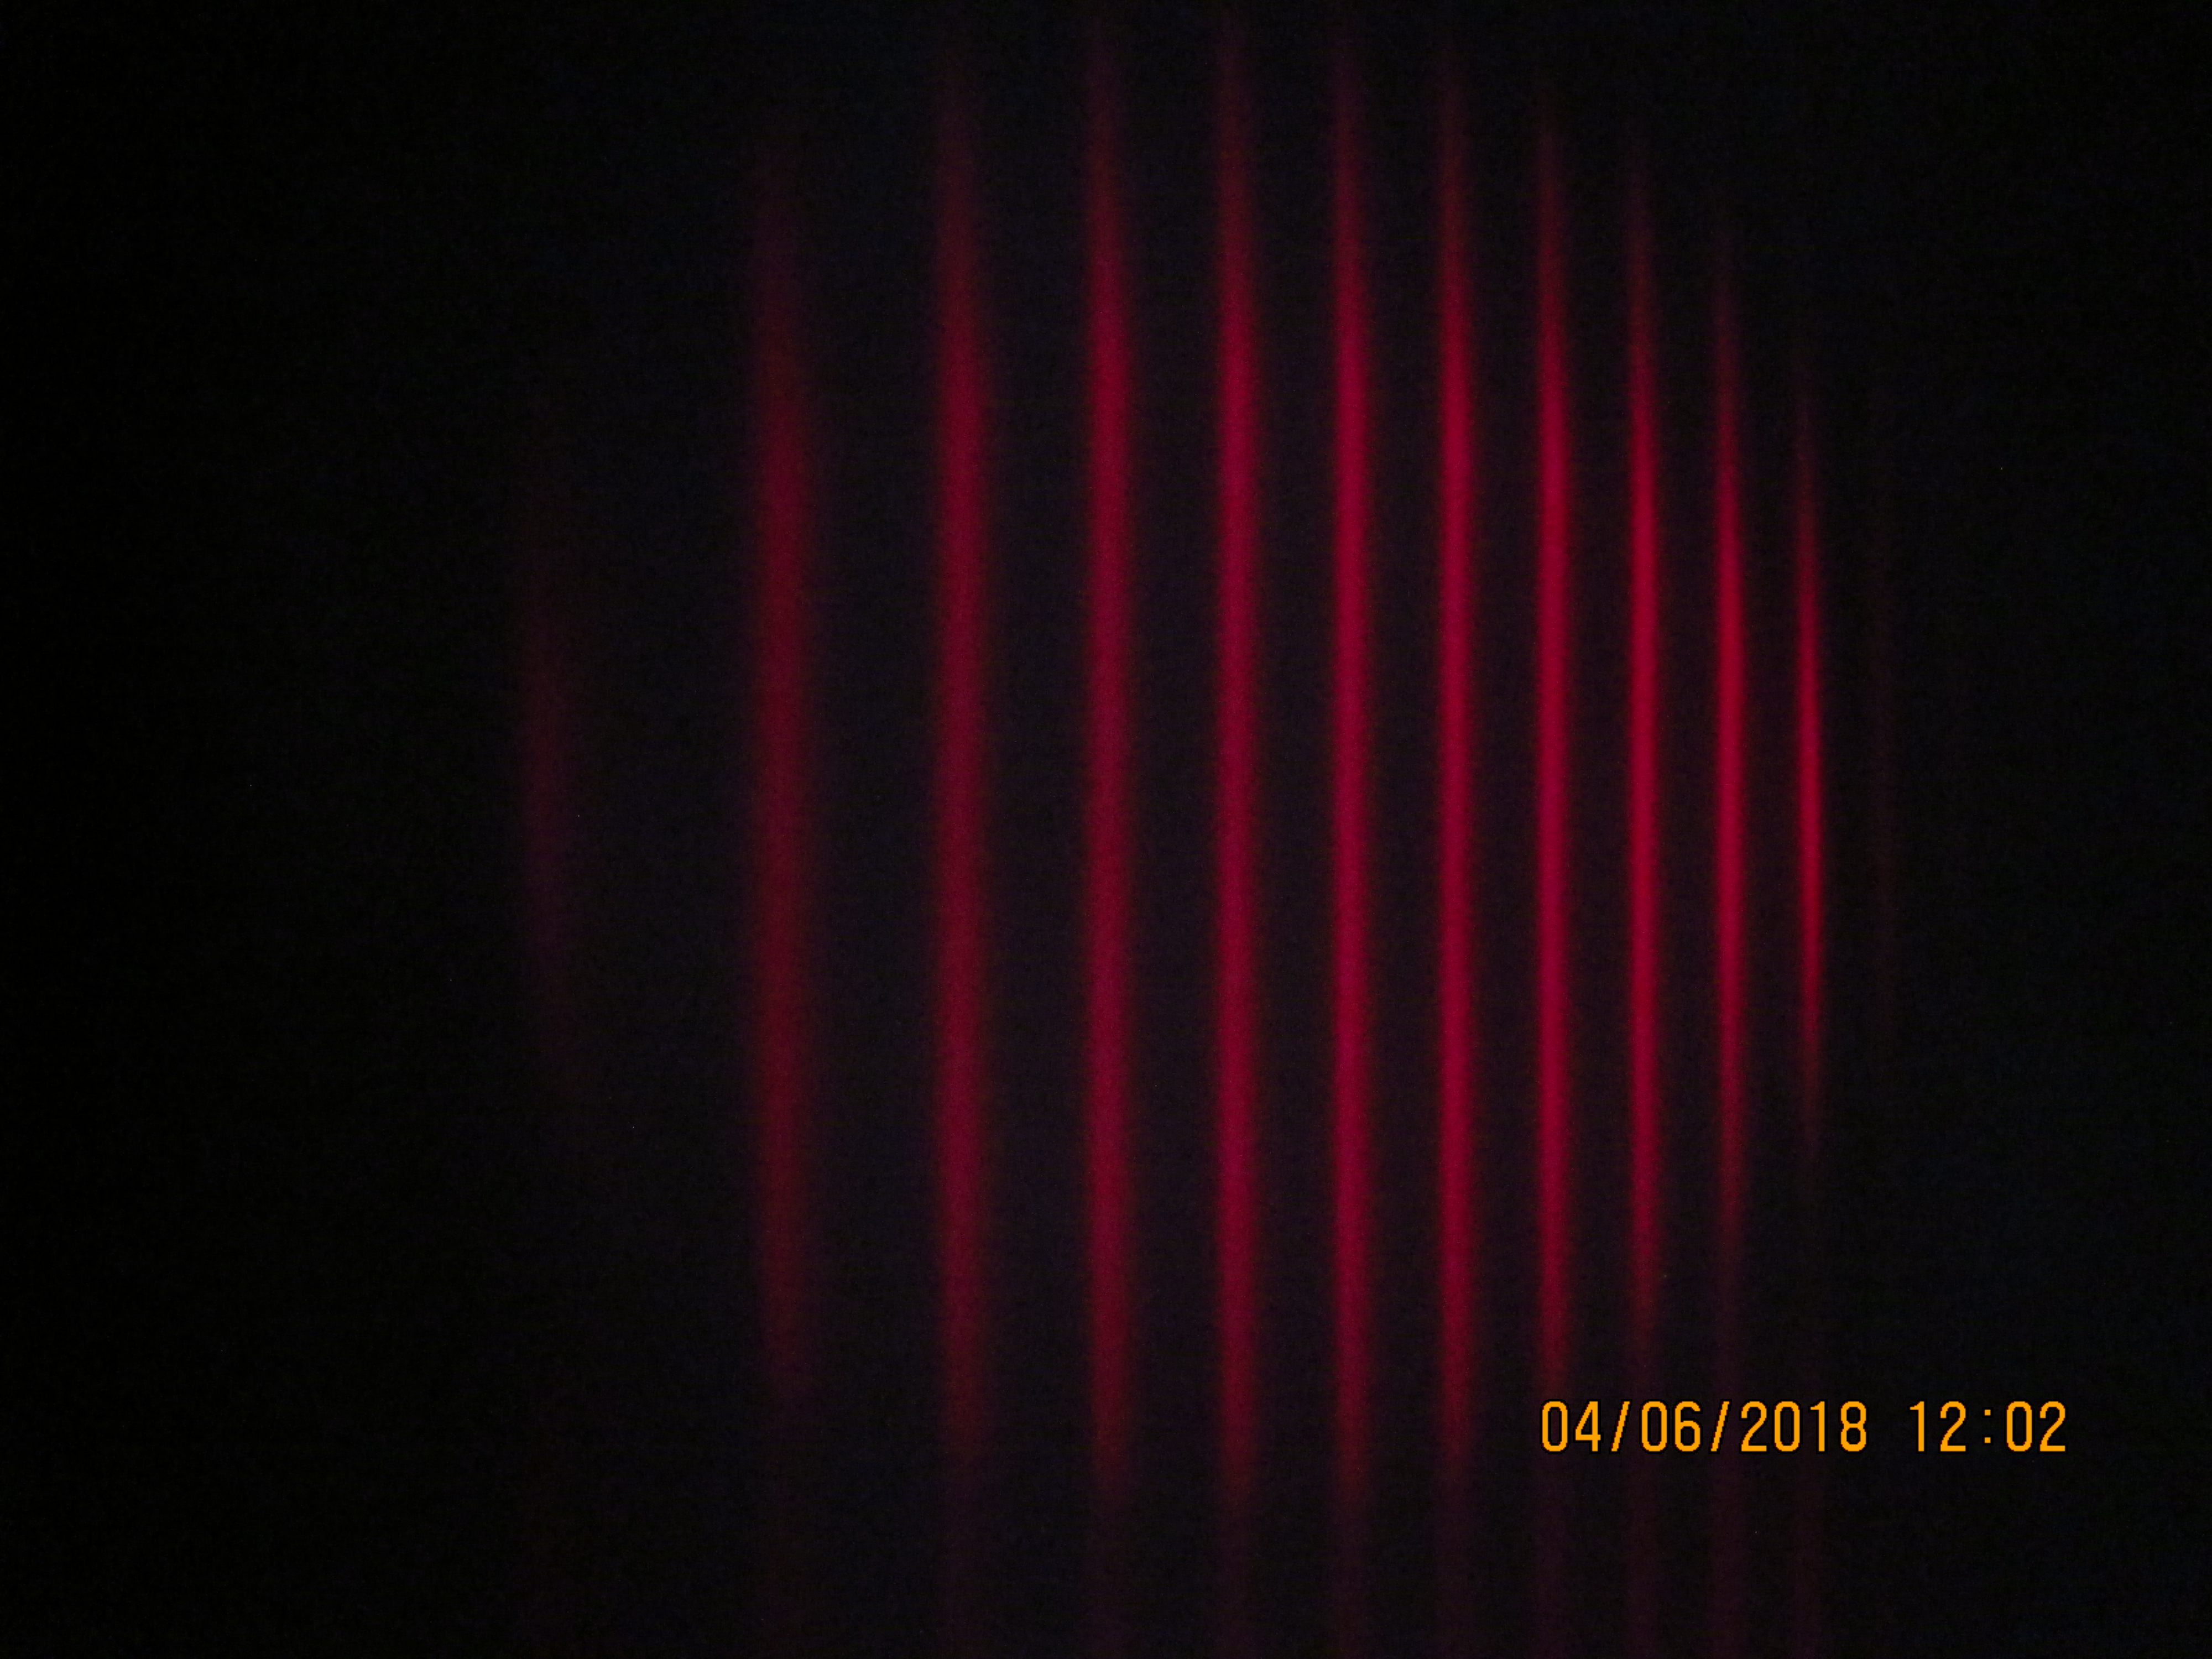
\includegraphics[width=\textwidth]{graphics/aufnahmen/IMG_1629.jpg}
    \caption{Aufnahme ohne Magnetfeld.}
  \end{subfigure}
  \begin{subfigure}{0.48\textwidth}
    \centering
    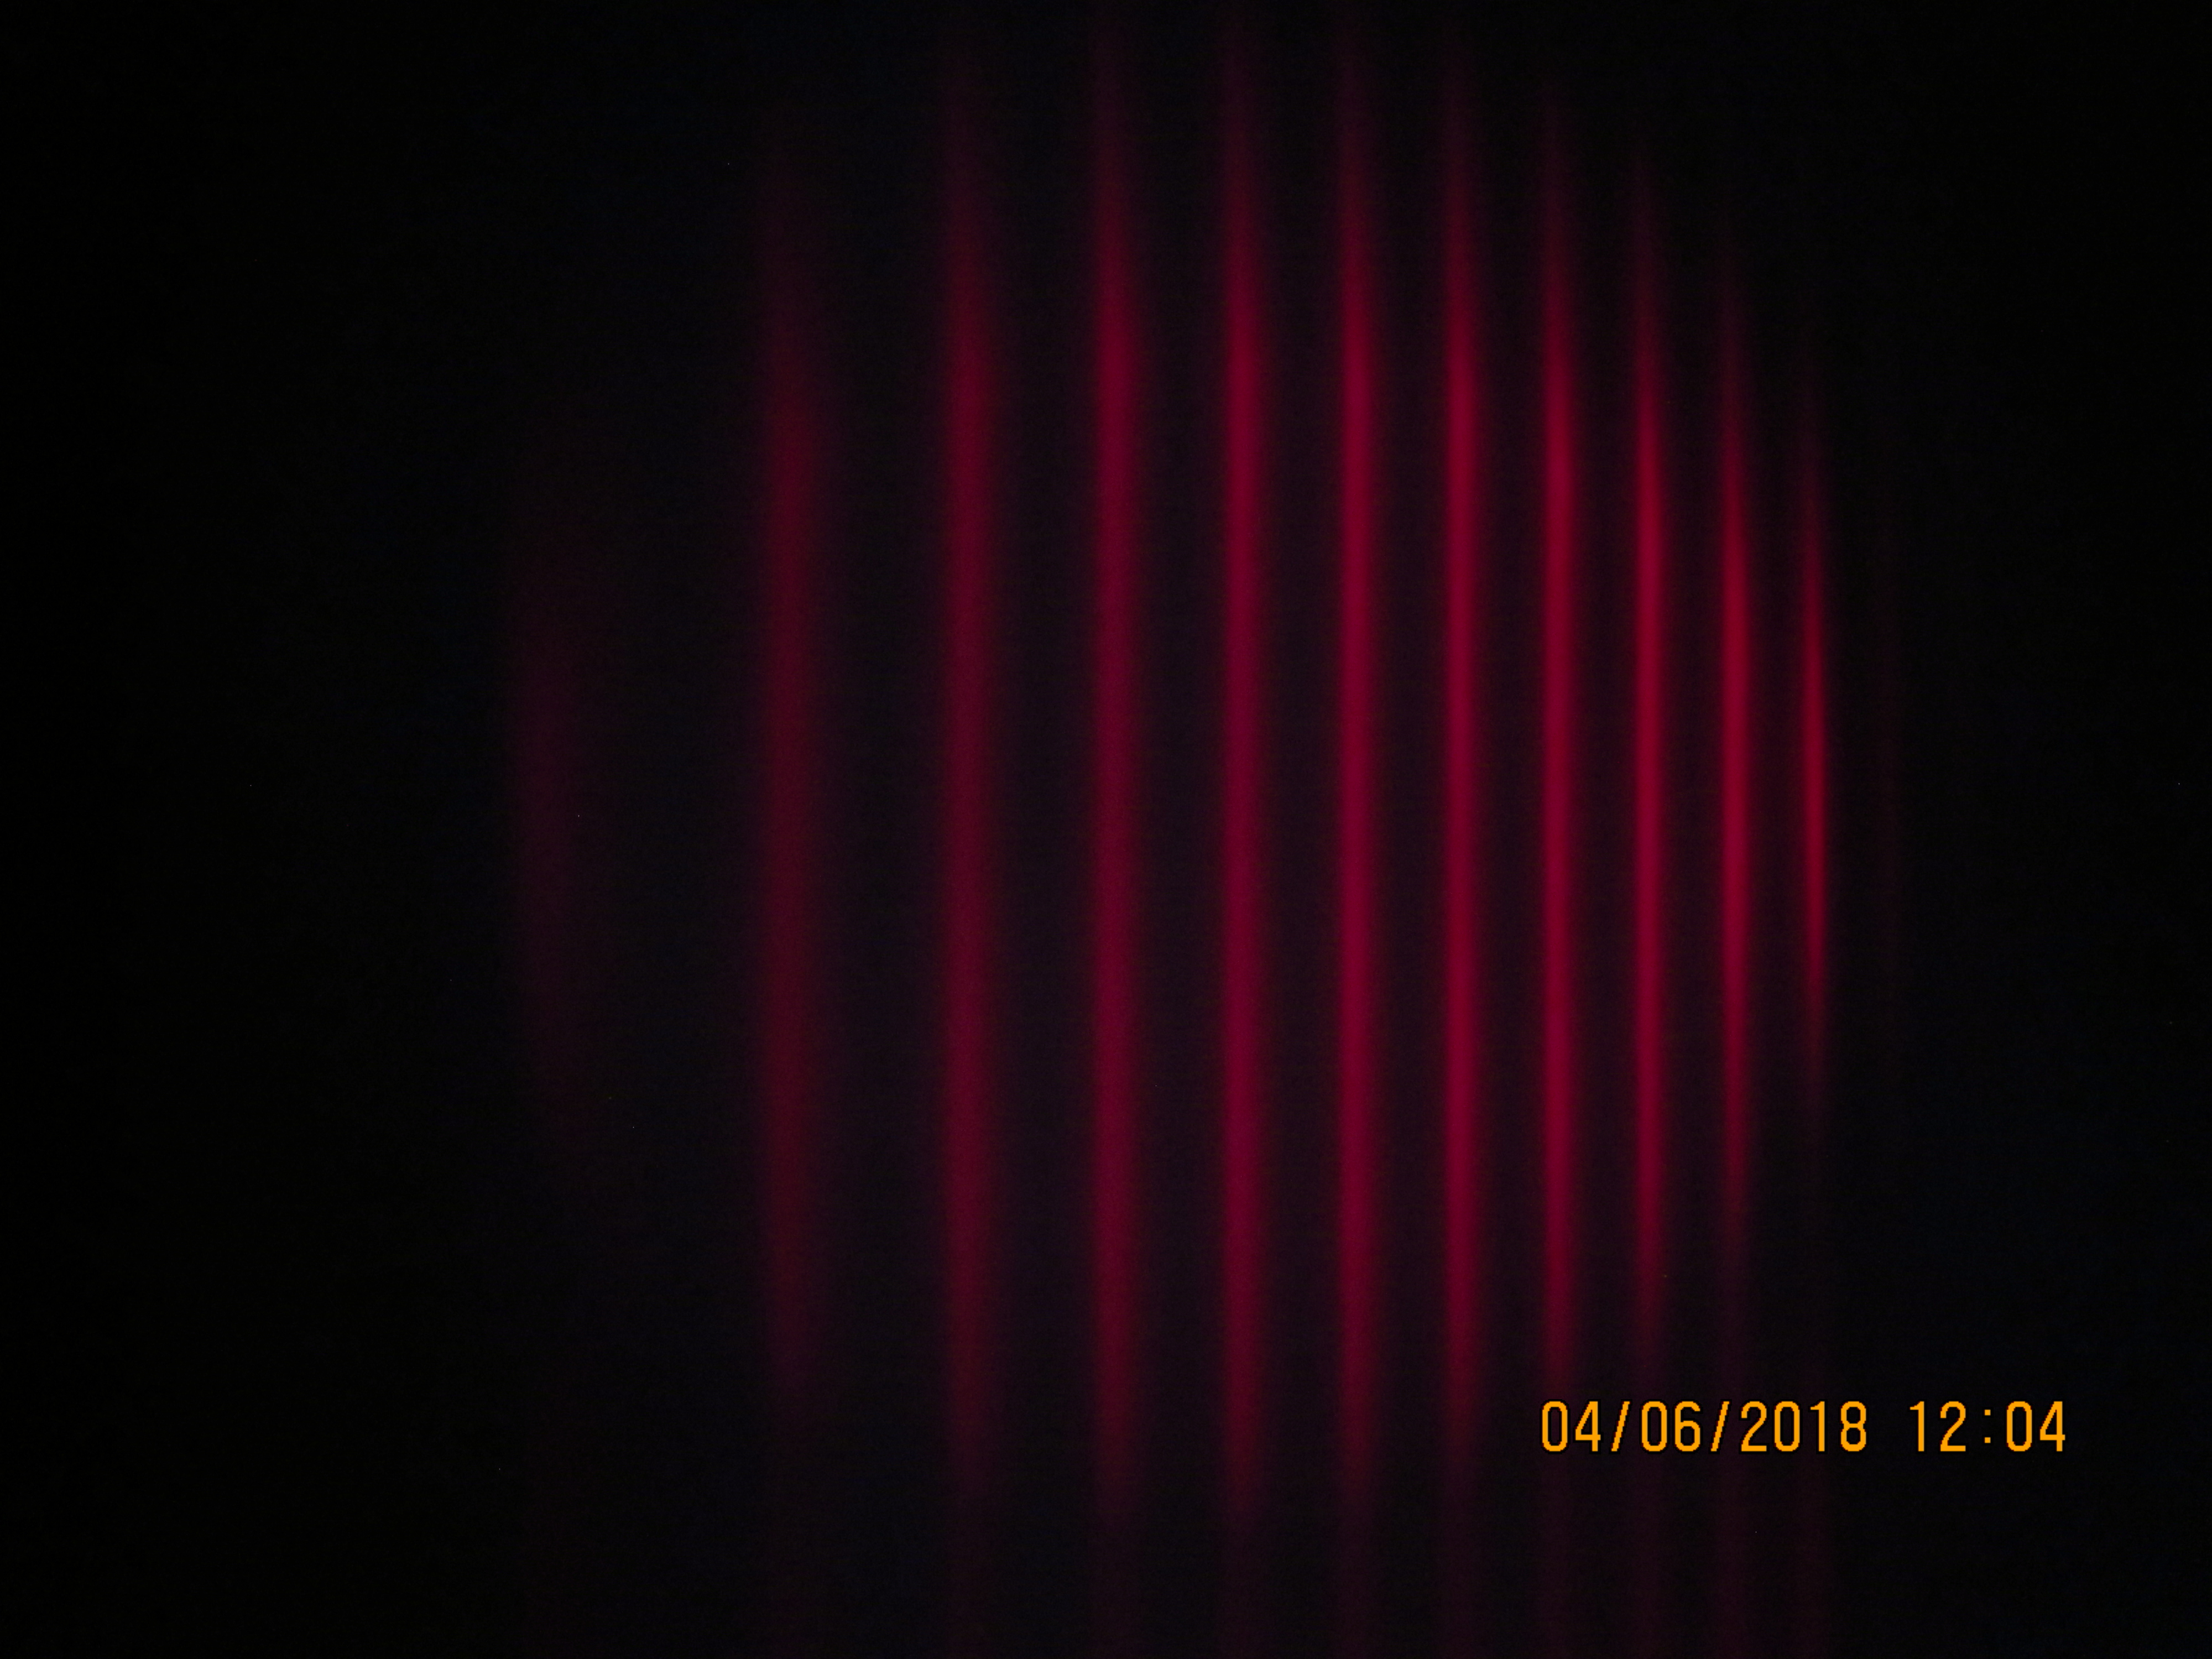
\includegraphics[width=\textwidth]{graphics/aufnahmen/IMG_1630.jpg}
    \caption{Aufnahme mit Magnetfeld.}
  \end{subfigure}
  \caption{Spektrallinien der roten $\pi$-Linie.}
  \label{fig:r_pi}
\end{figure}

Die Messungen der roten $\sigma$-Linie ergeben die Bilder \ref{fig:r_sigma} und \ref{fig:r_sigma_B}. Die gemessenen Abstände, die nach \eqref{eq:versch} berechnete Verschiebung
und die daraus folgenden Landé-Faktoren sind in Tabelle \ref{tab:r_sigma} dargestellt. Die verwendete Magnetfeldstärke ist $\SI{597 \pm 6}{mT}$ und es ergibt sich der mittlere
Landé-Faktor $g = \num{0.981 \pm  0.009}$.

\begin{figure}
  \centering
  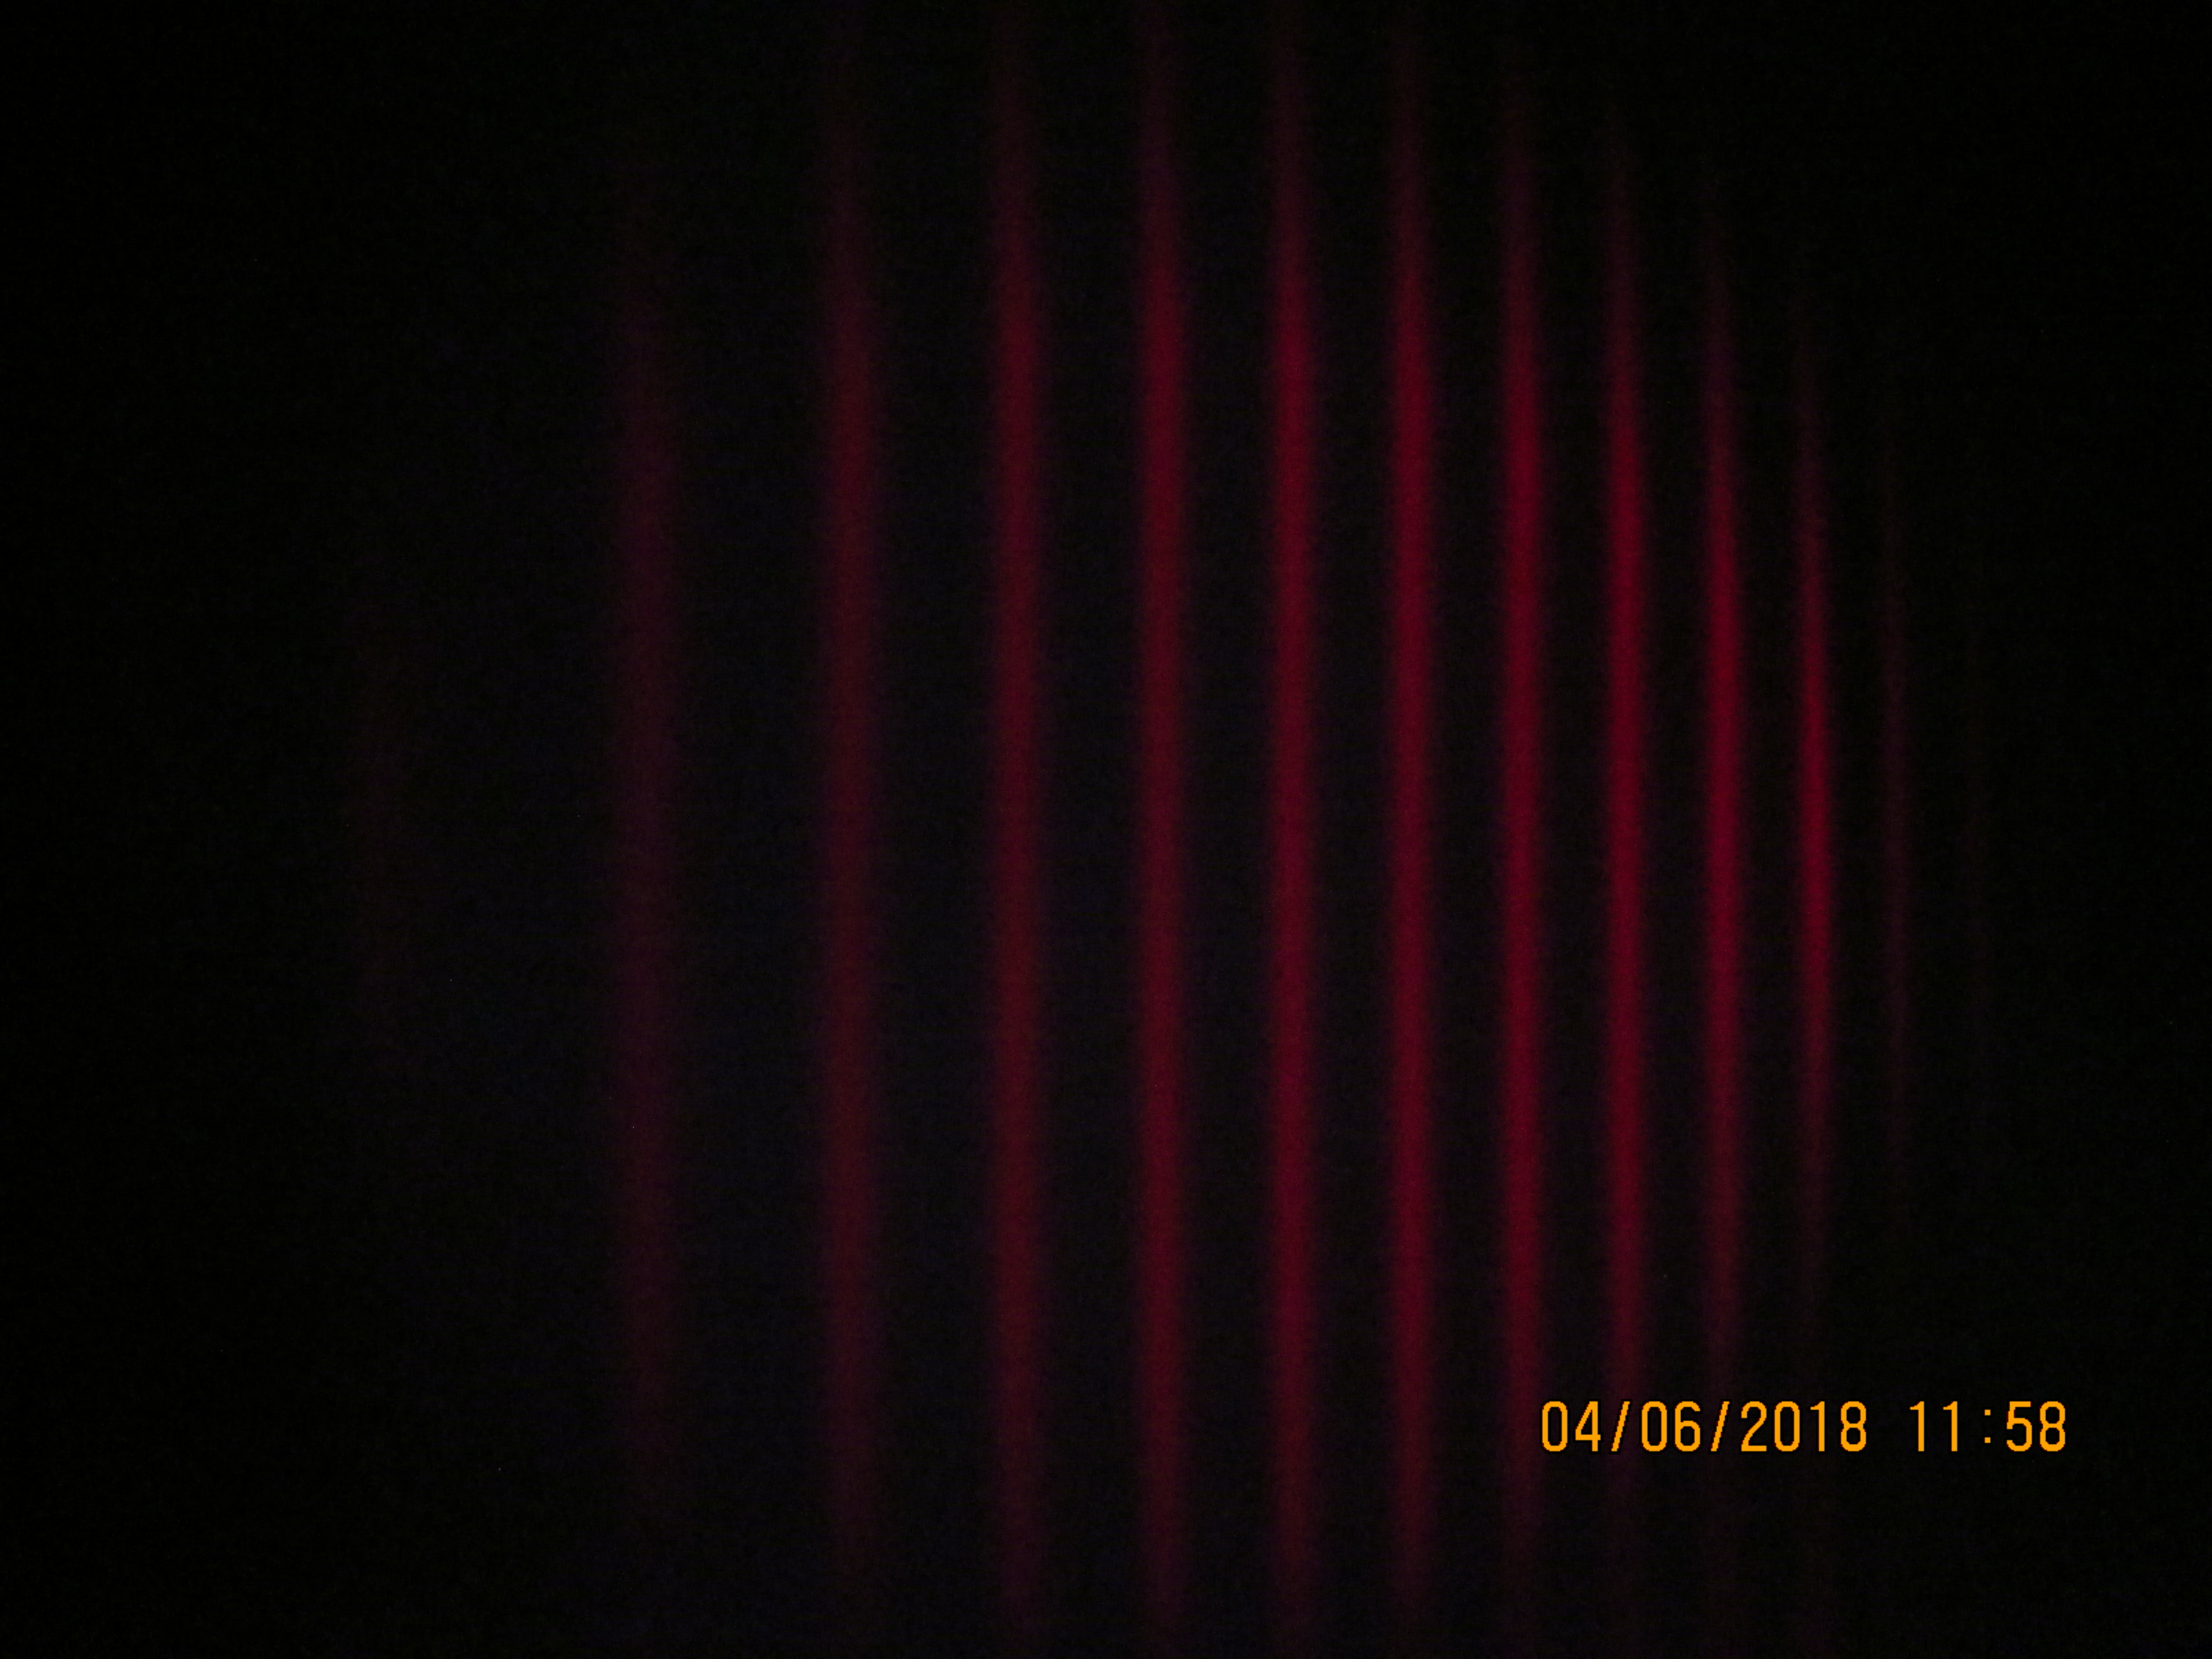
\includegraphics[width=0.95\textwidth]{graphics/auswertung/IMG_1627.png}
  \caption{Rote $\sigma$-Linie ohne Magnetfeld.}
  \label{fig:r_sigma}
\end{figure}
\begin{figure}
  \centering
  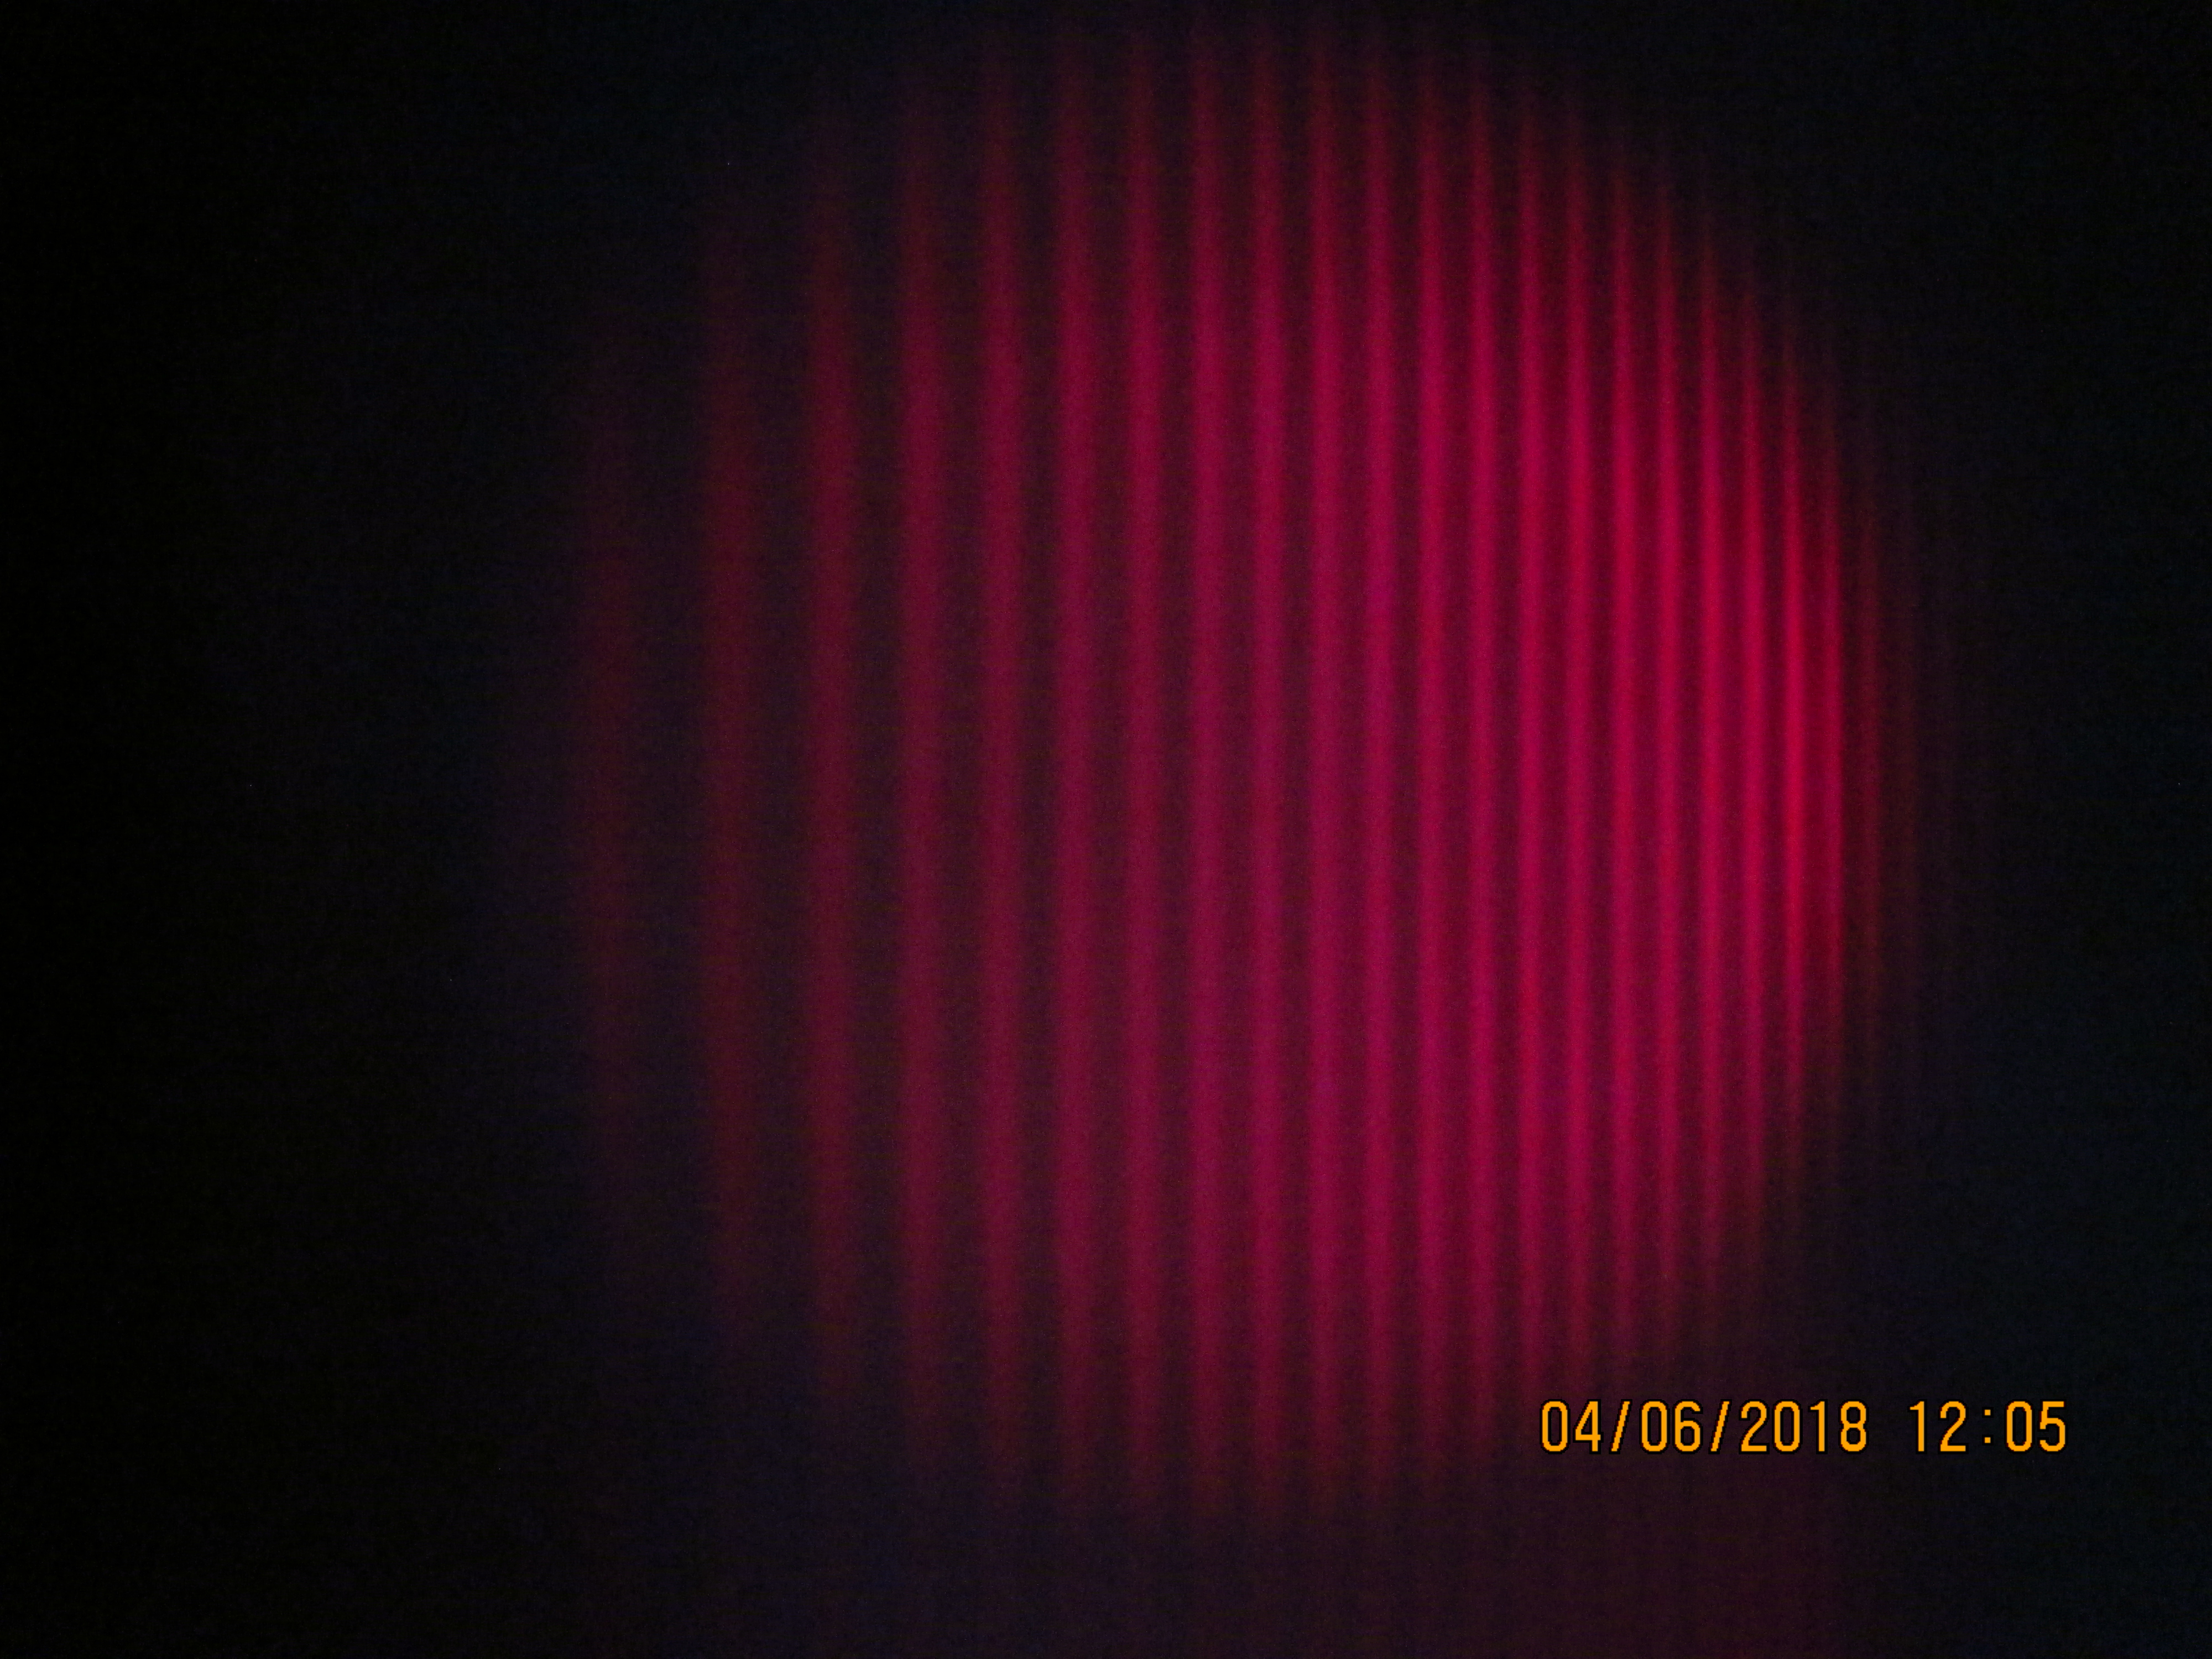
\includegraphics[width=0.95\textwidth]{graphics/auswertung/IMG_1632.png}
  \caption{Rote $\sigma$-Linie mit Magnetfeld.}
  \label{fig:r_sigma_B}
\end{figure}

\begin{table}
  \centering
  \caption{Messwerte der roten $\sigma$-Linie.}
  \label{tab:r_sigma}
  \begin{tabular}{S[table-format=3] S[table-format=3] S[table-format=2.3] S[table-format=1.3] @{${}\pm{}$} S[table-format=1.3]}
    \toprule
    {$\upD s \:/\: $px} & {$\symup{\delta} s \:/\: $px} & {$\symup{\delta}\lambda \:/\: $pm} & \multicolumn{2}{c}{Landé-Faktor $g$} \\
    \midrule
    367 & 192 & 12.794 & 1.108 & 0.010 \\
    304 & 150 & 12.067 & 1.045 & 0.010 \\
    261 & 126 & 11.806 & 1.022 & 0.010 \\
    236 & 106 & 10.984 & 0.951 & 0.009 \\
    213 &  94 & 10.792 & 0.934 & 0.009 \\
    199 &  90 & 11.060 & 0.958 & 0.009 \\
    190 &  84 & 10.812 & 0.936 & 0.009 \\
    177 &  76 & 10.500 & 0.909 & 0.009 \\
    167 &  76 & 11.129 & 0.964 & 0.009 \\
    \bottomrule
  \end{tabular}
\end{table}
%
\ \\
Bei der blauen $\pi$-Linie und der blauen $\sigma$-Linie wird analog verfahren. Die $\pi$-Linie ergibt die
Bilder \ref{fig:b_pi} und \ref{fig:b_pi_B} und die Messwerte in Tabelle \ref{tab:b_pi}. Gemessen wurde bei einem
Magnetfeld von $\SI{1002 \pm 8}{mT}$ und für den Landé-Faktor ergibt sich der Mittelwert $g = \num{0.525 \pm 0.004}$.

Die Bilder \ref{fig:b_sigma} und \ref{fig:b_sigma_B} der $\sigma$-Linie ergeben die Messwerte aus Tabelle \ref{tab:b_sigma} bei
einem Magnetfeld von $\SI{365 \pm 5}{mT}$. Es ergibt sich der Faktor $g = \num{1.39  \pm  0.02}$.

\begin{figure}
  \centering
  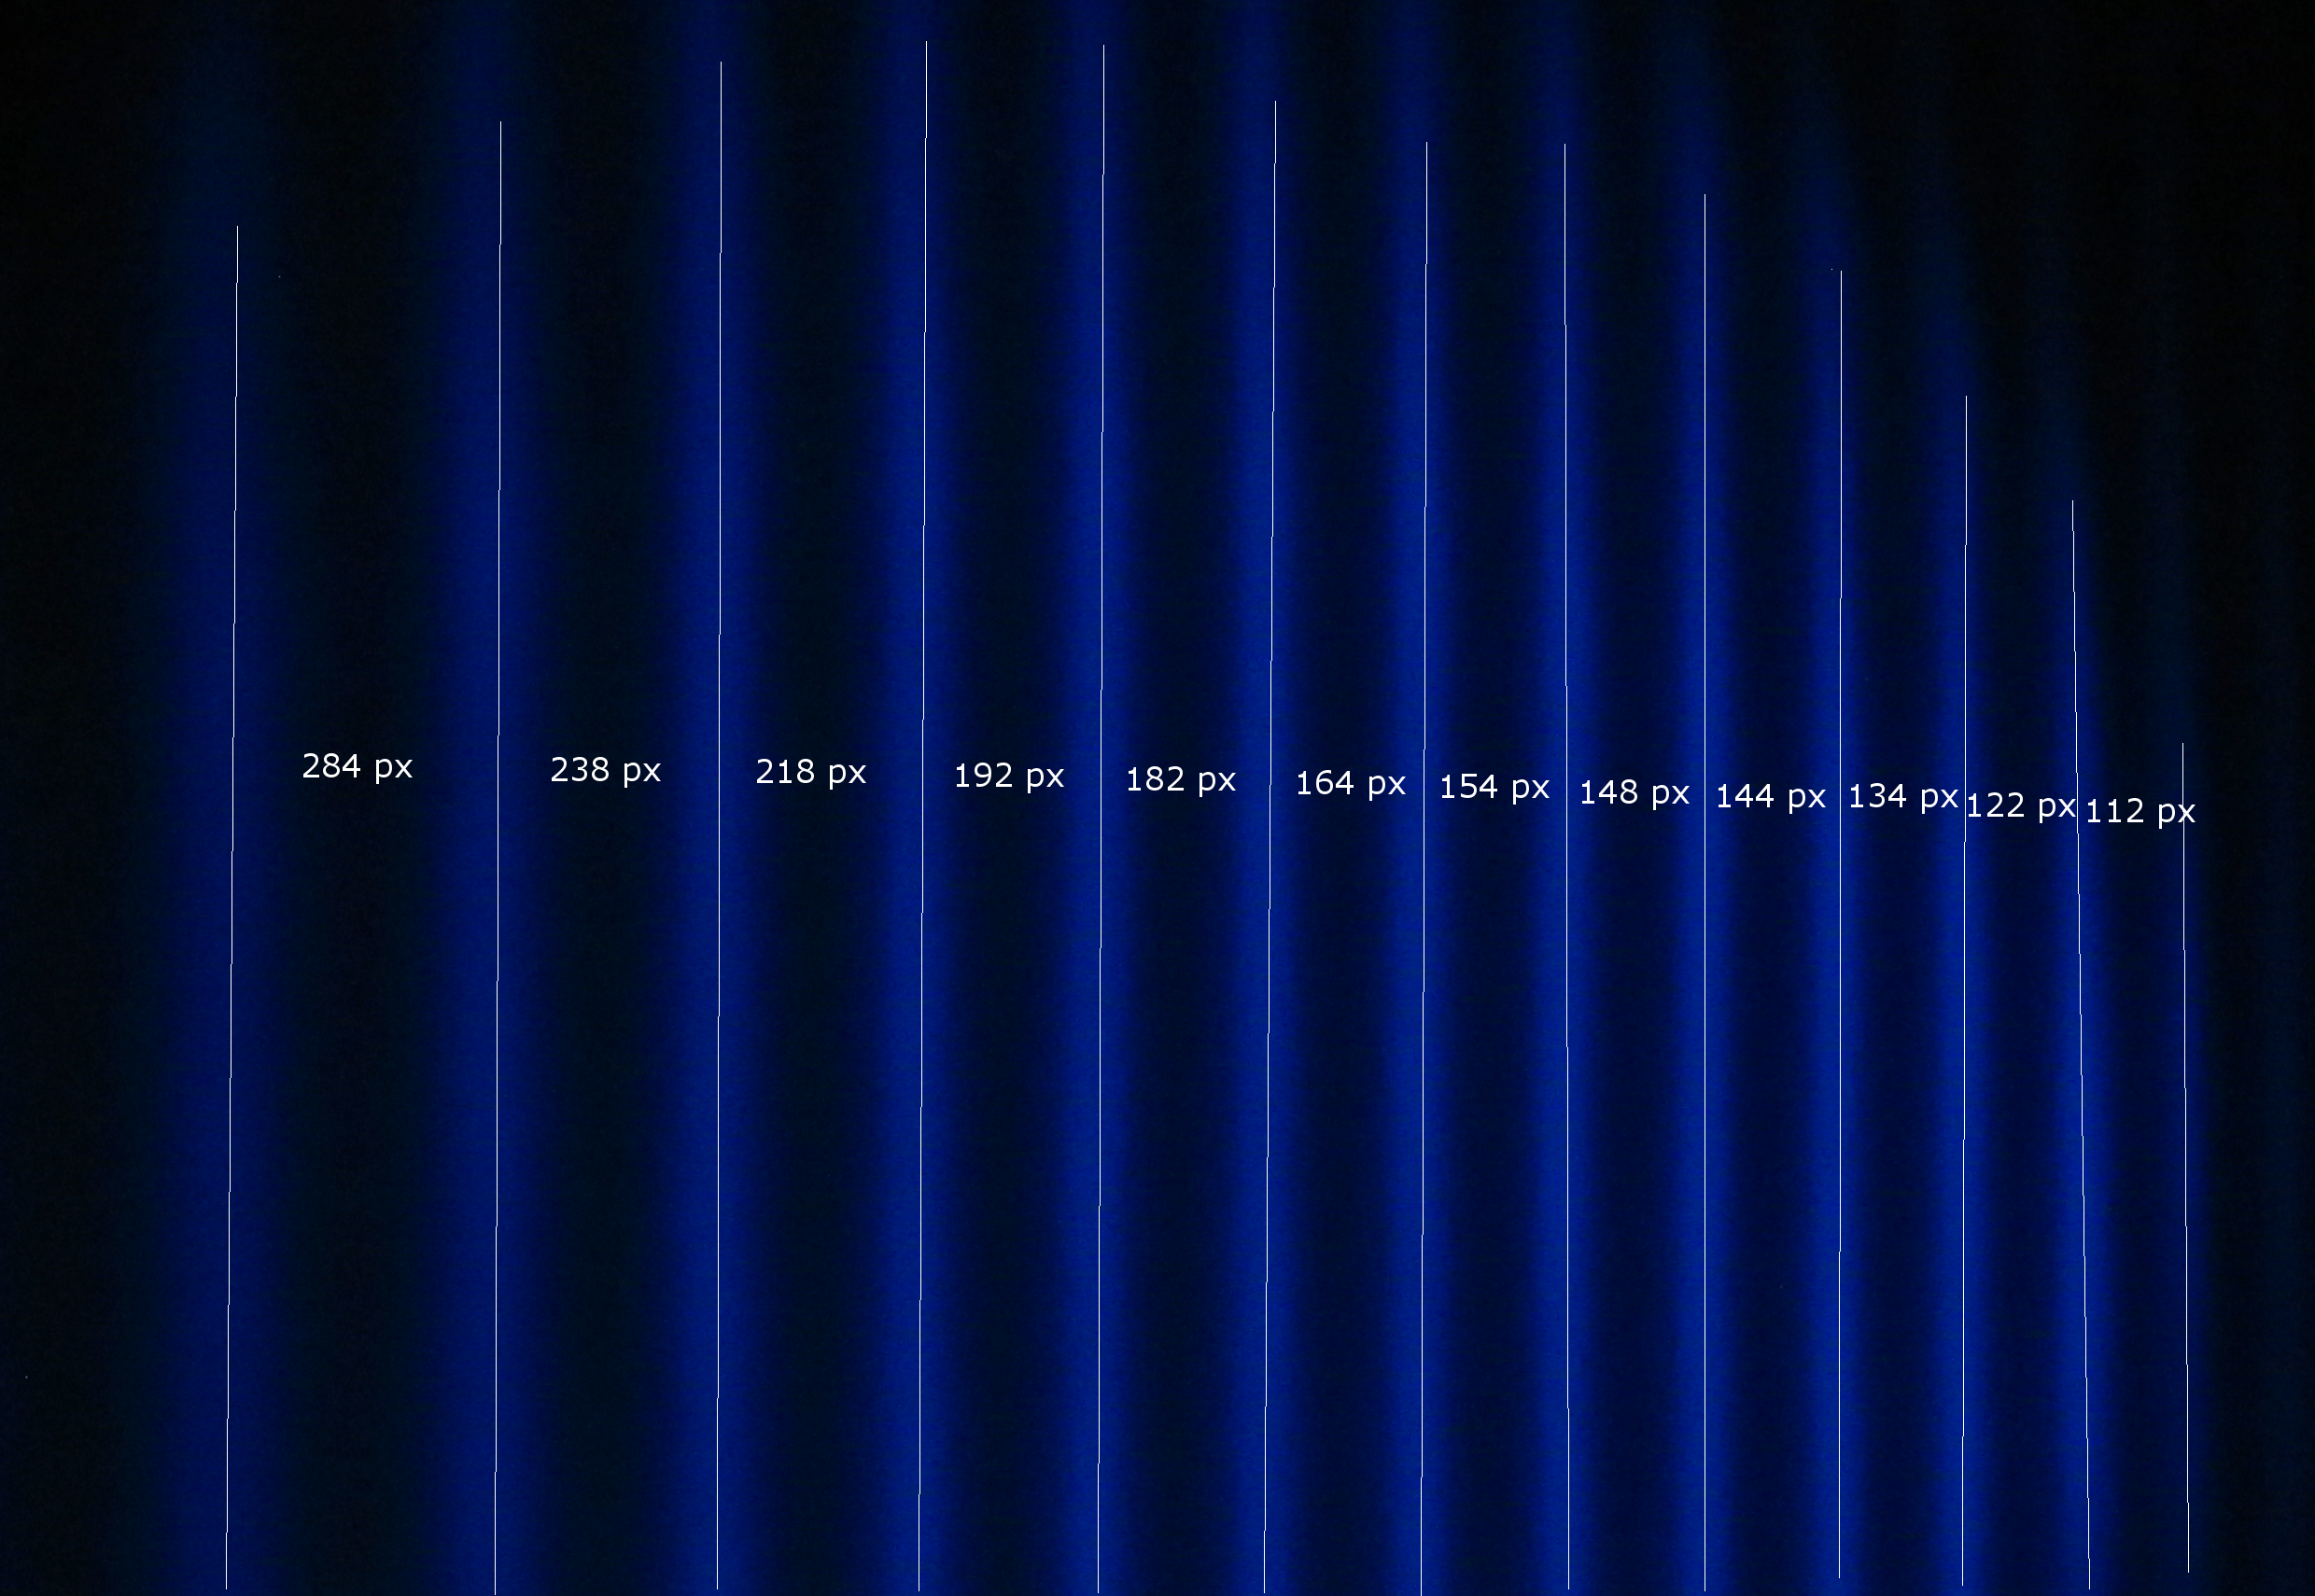
\includegraphics[width=0.95\textwidth]{graphics/auswertung/IMG_1635.png}
  \caption{Blaue $\pi$-Linie ohne Magnetfeld.}
  \label{fig:b_pi}
\end{figure}
\begin{figure}
  \centering
  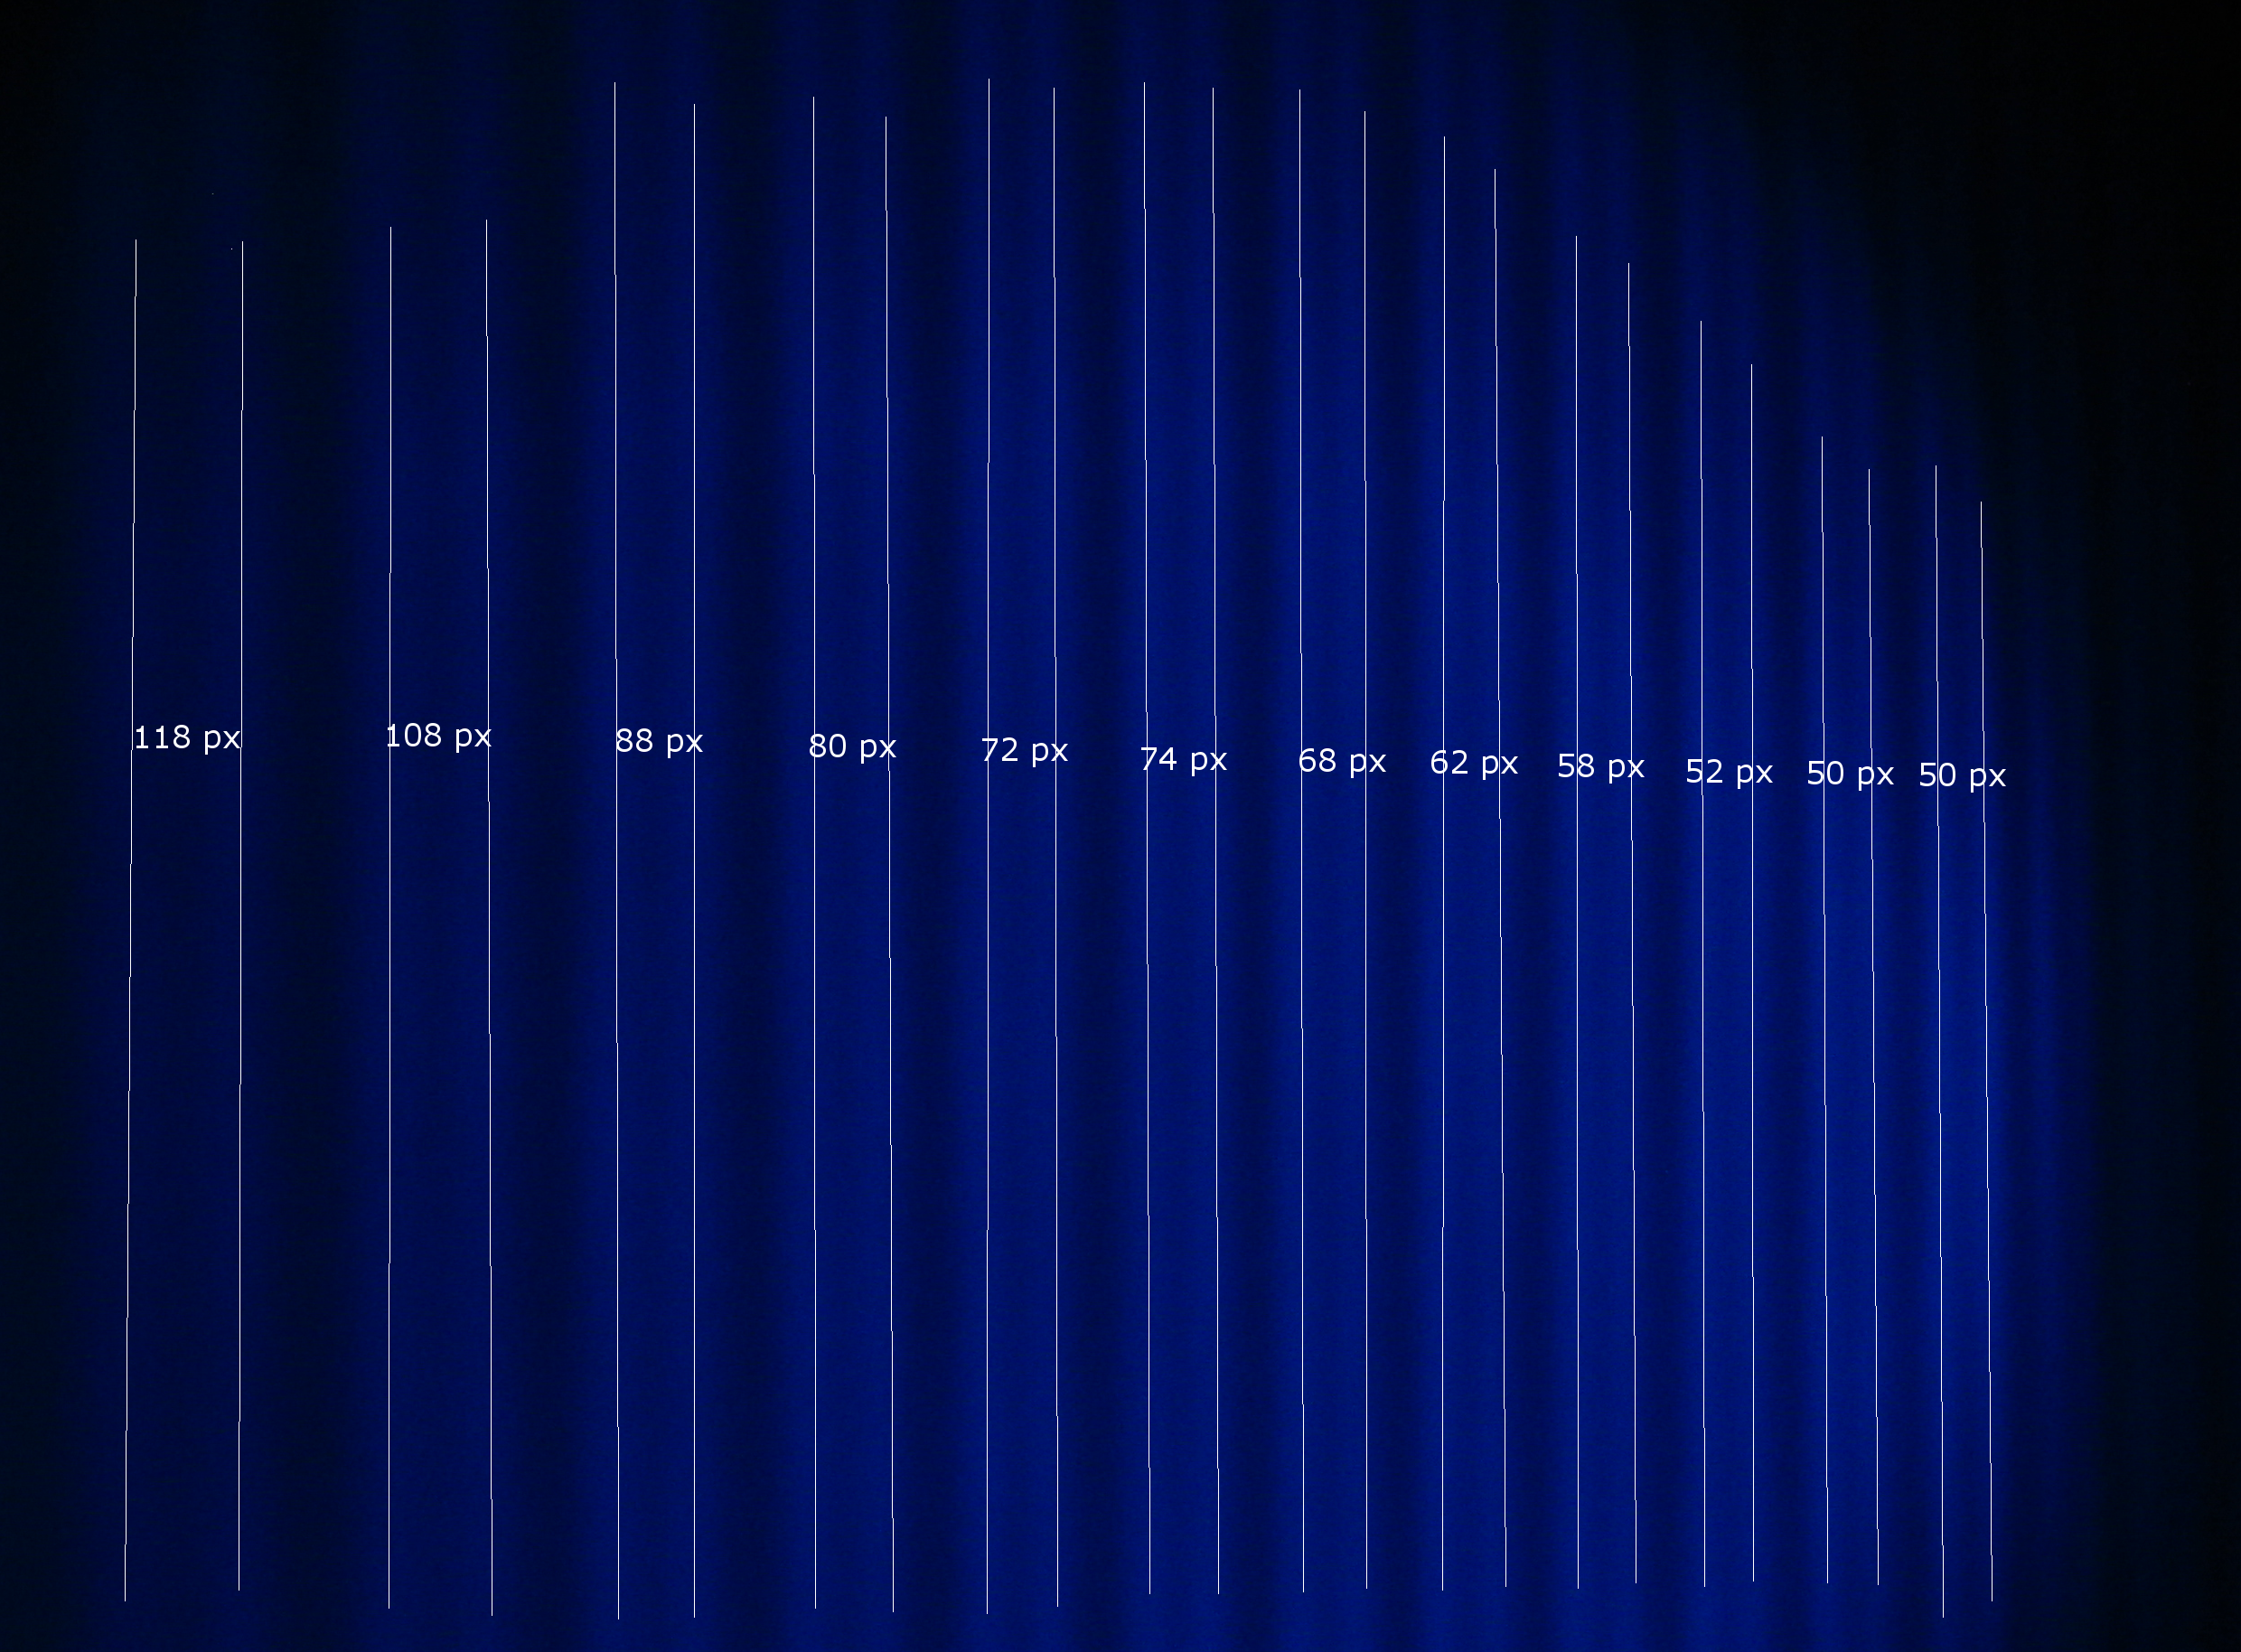
\includegraphics[width=0.95\textwidth]{graphics/auswertung/IMG_1644.png}
  \caption{Blaue $\pi$-Linie mit Magnetfeld.}
  \label{fig:b_pi_B}
\end{figure}

\begin{table}
  \centering
  \caption{Messwerte der blauen $\pi$-Linie.}
  \label{tab:b_pi}
  \begin{tabular}{S[table-format=3] S[table-format=3] S[table-format=2.3] S[table-format=1.3] @{${}\pm{}$} S[table-format=1.3]}
    \toprule
    {$\upD s \:/\: $px} & {$\symup{\delta} s \:/\: $px} & {$\symup{\delta}\lambda \:/\: $pm} & \multicolumn{2}{c}{Landé-Faktor $g$} \\
    \midrule
    284 & 118 & 5.599 & 0.519 & 0.004 \\
    238 & 108 & 6.115 & 0.567 & 0.004 \\
    218 &  88 & 5.439 & 0.505 & 0.004 \\
    192 &  80 & 5.615 & 0.521 & 0.004 \\
    182 &  72 & 5.331 & 0.495 & 0.004 \\
    164 &  74 & 6.080 & 0.564 & 0.004 \\
    154 &  68 & 5.950 & 0.552 & 0.004 \\
    148 &  62 & 5.645 & 0.524 & 0.004 \\
    144 &  58 & 5.427 & 0.503 & 0.004 \\
    134 &  52 & 5.229 & 0.485 & 0.004 \\
    122 &  50 & 5.523 & 0.512 & 0.004 \\
    112 &  50 & 6.016 & 0.558 & 0.004 \\
    \bottomrule
  \end{tabular}
\end{table}


\begin{figure}
  \centering
  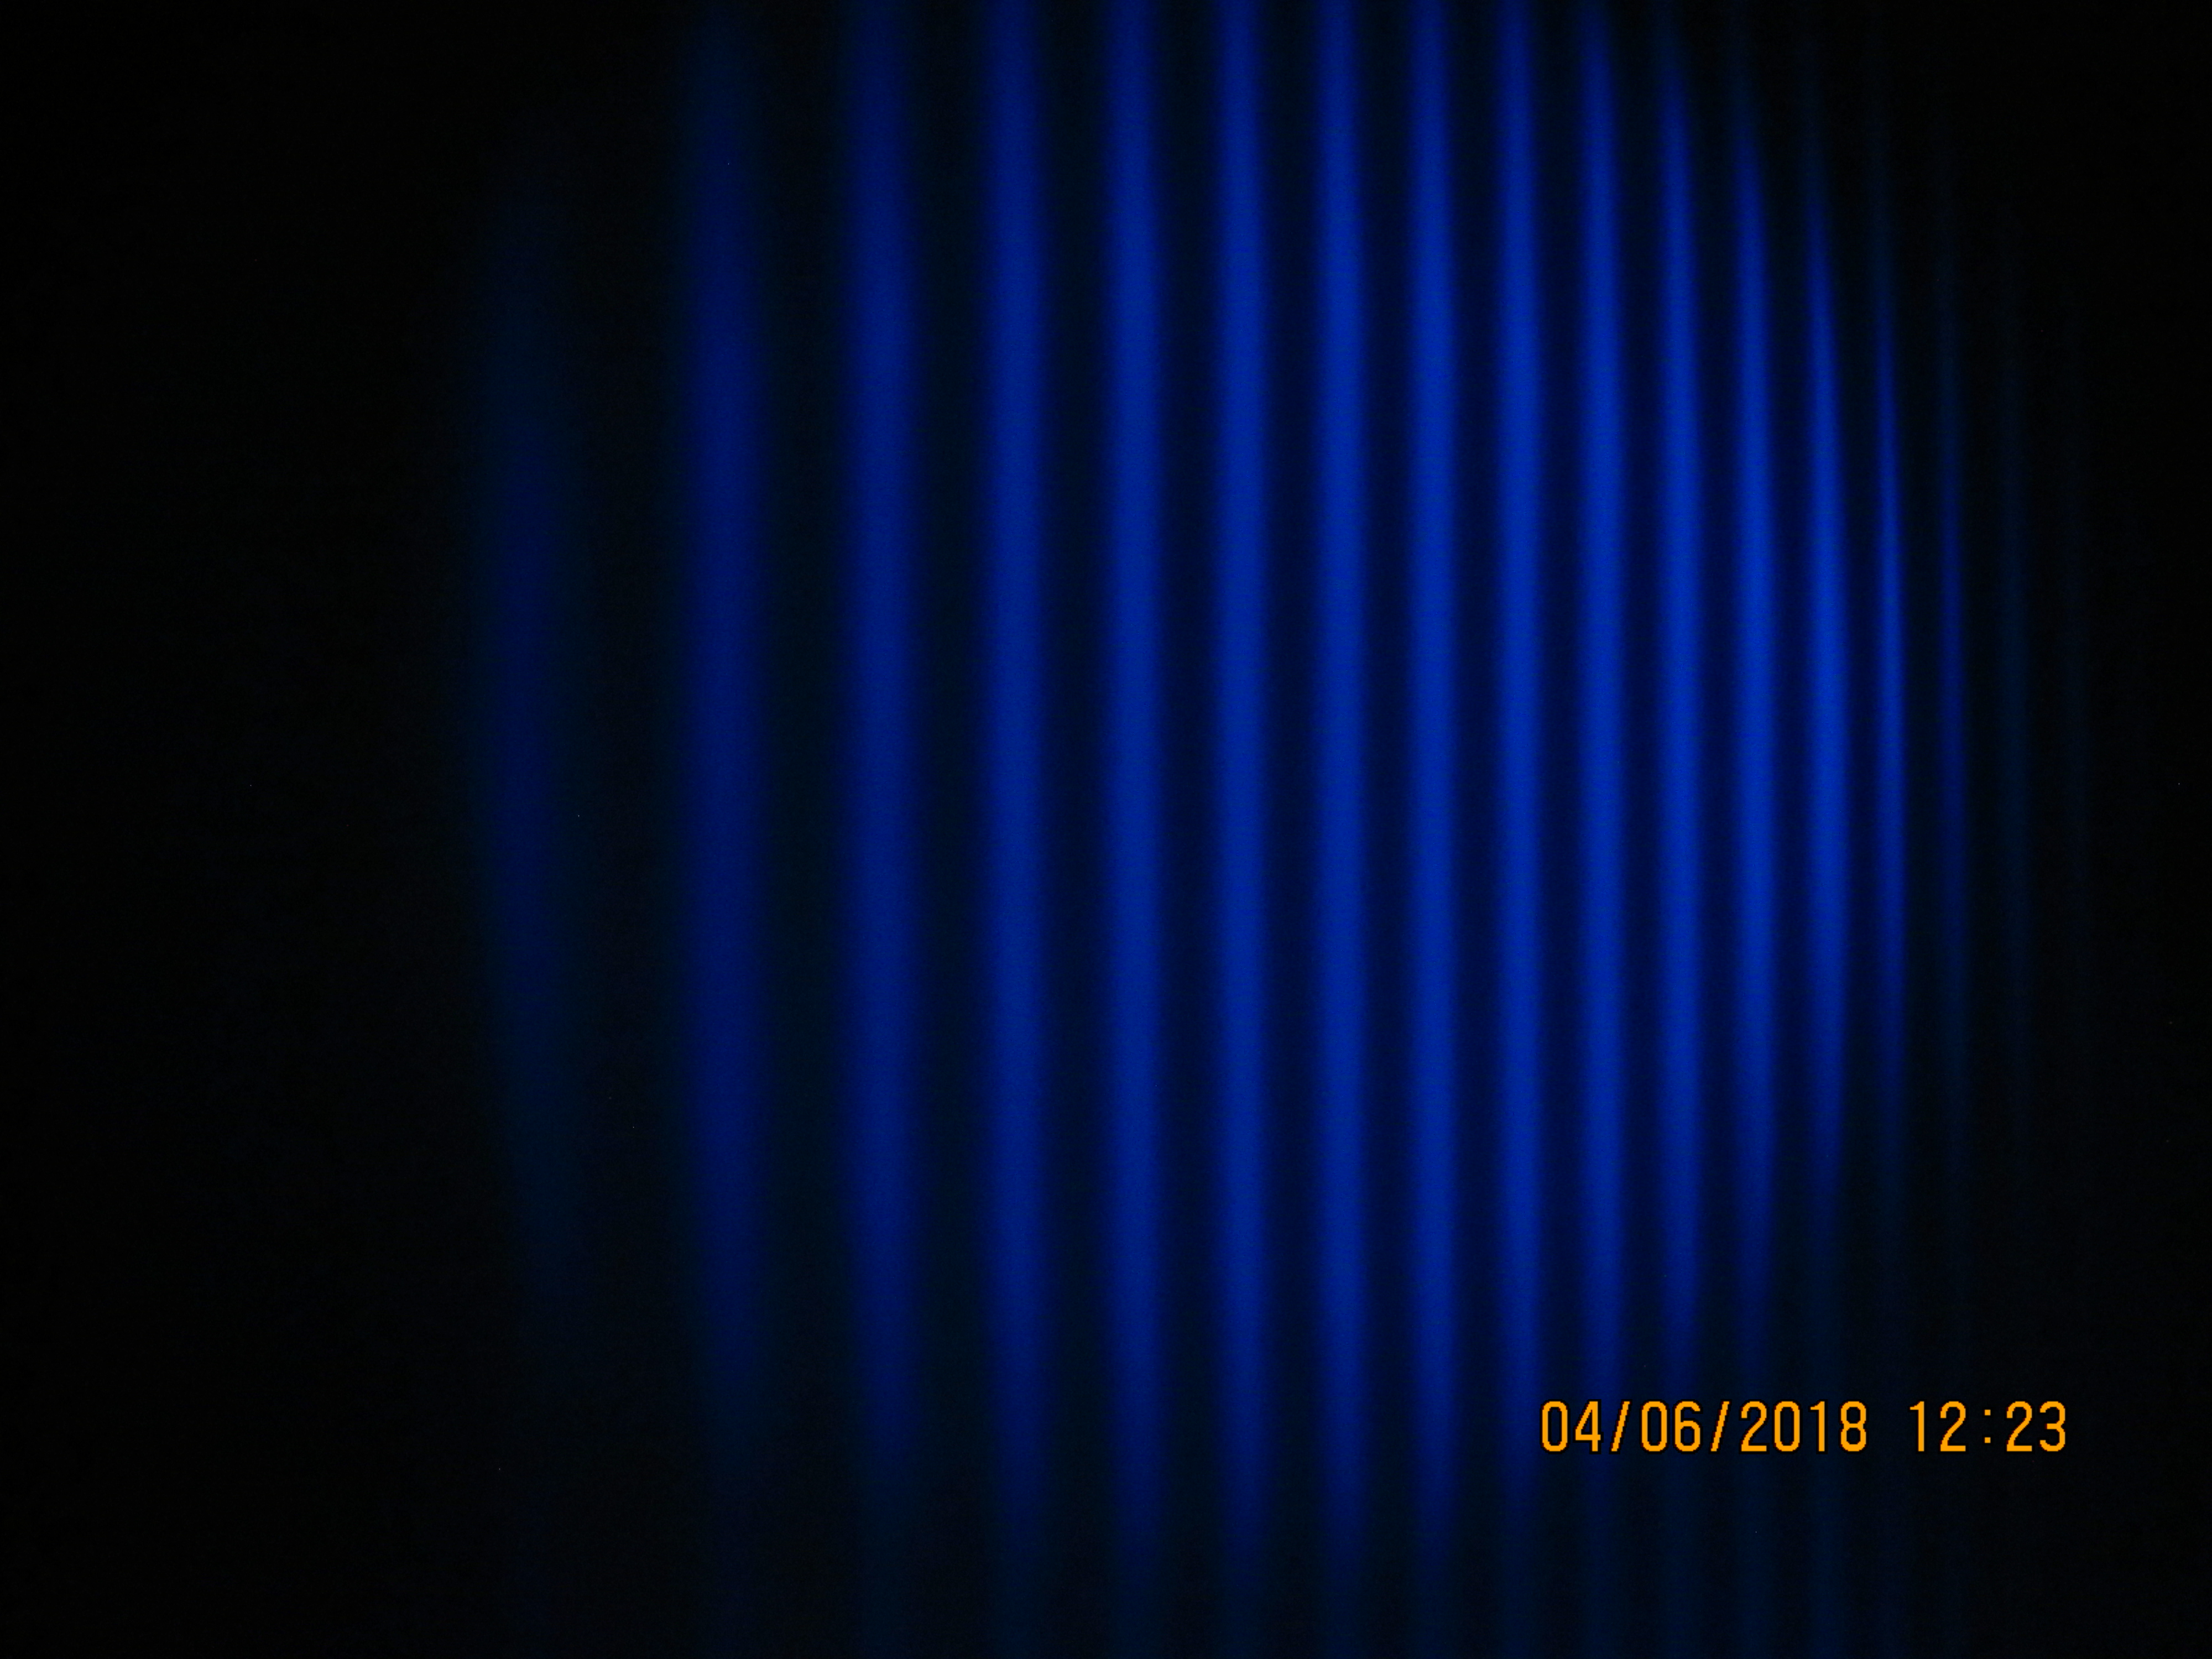
\includegraphics[width=0.95\textwidth]{graphics/auswertung/IMG_1637.png}
  \caption{Blaue $\sigma$-Linie ohne Magnetfeld.}
  \label{fig:b_sigma}
\end{figure}
\begin{figure}
  \centering
  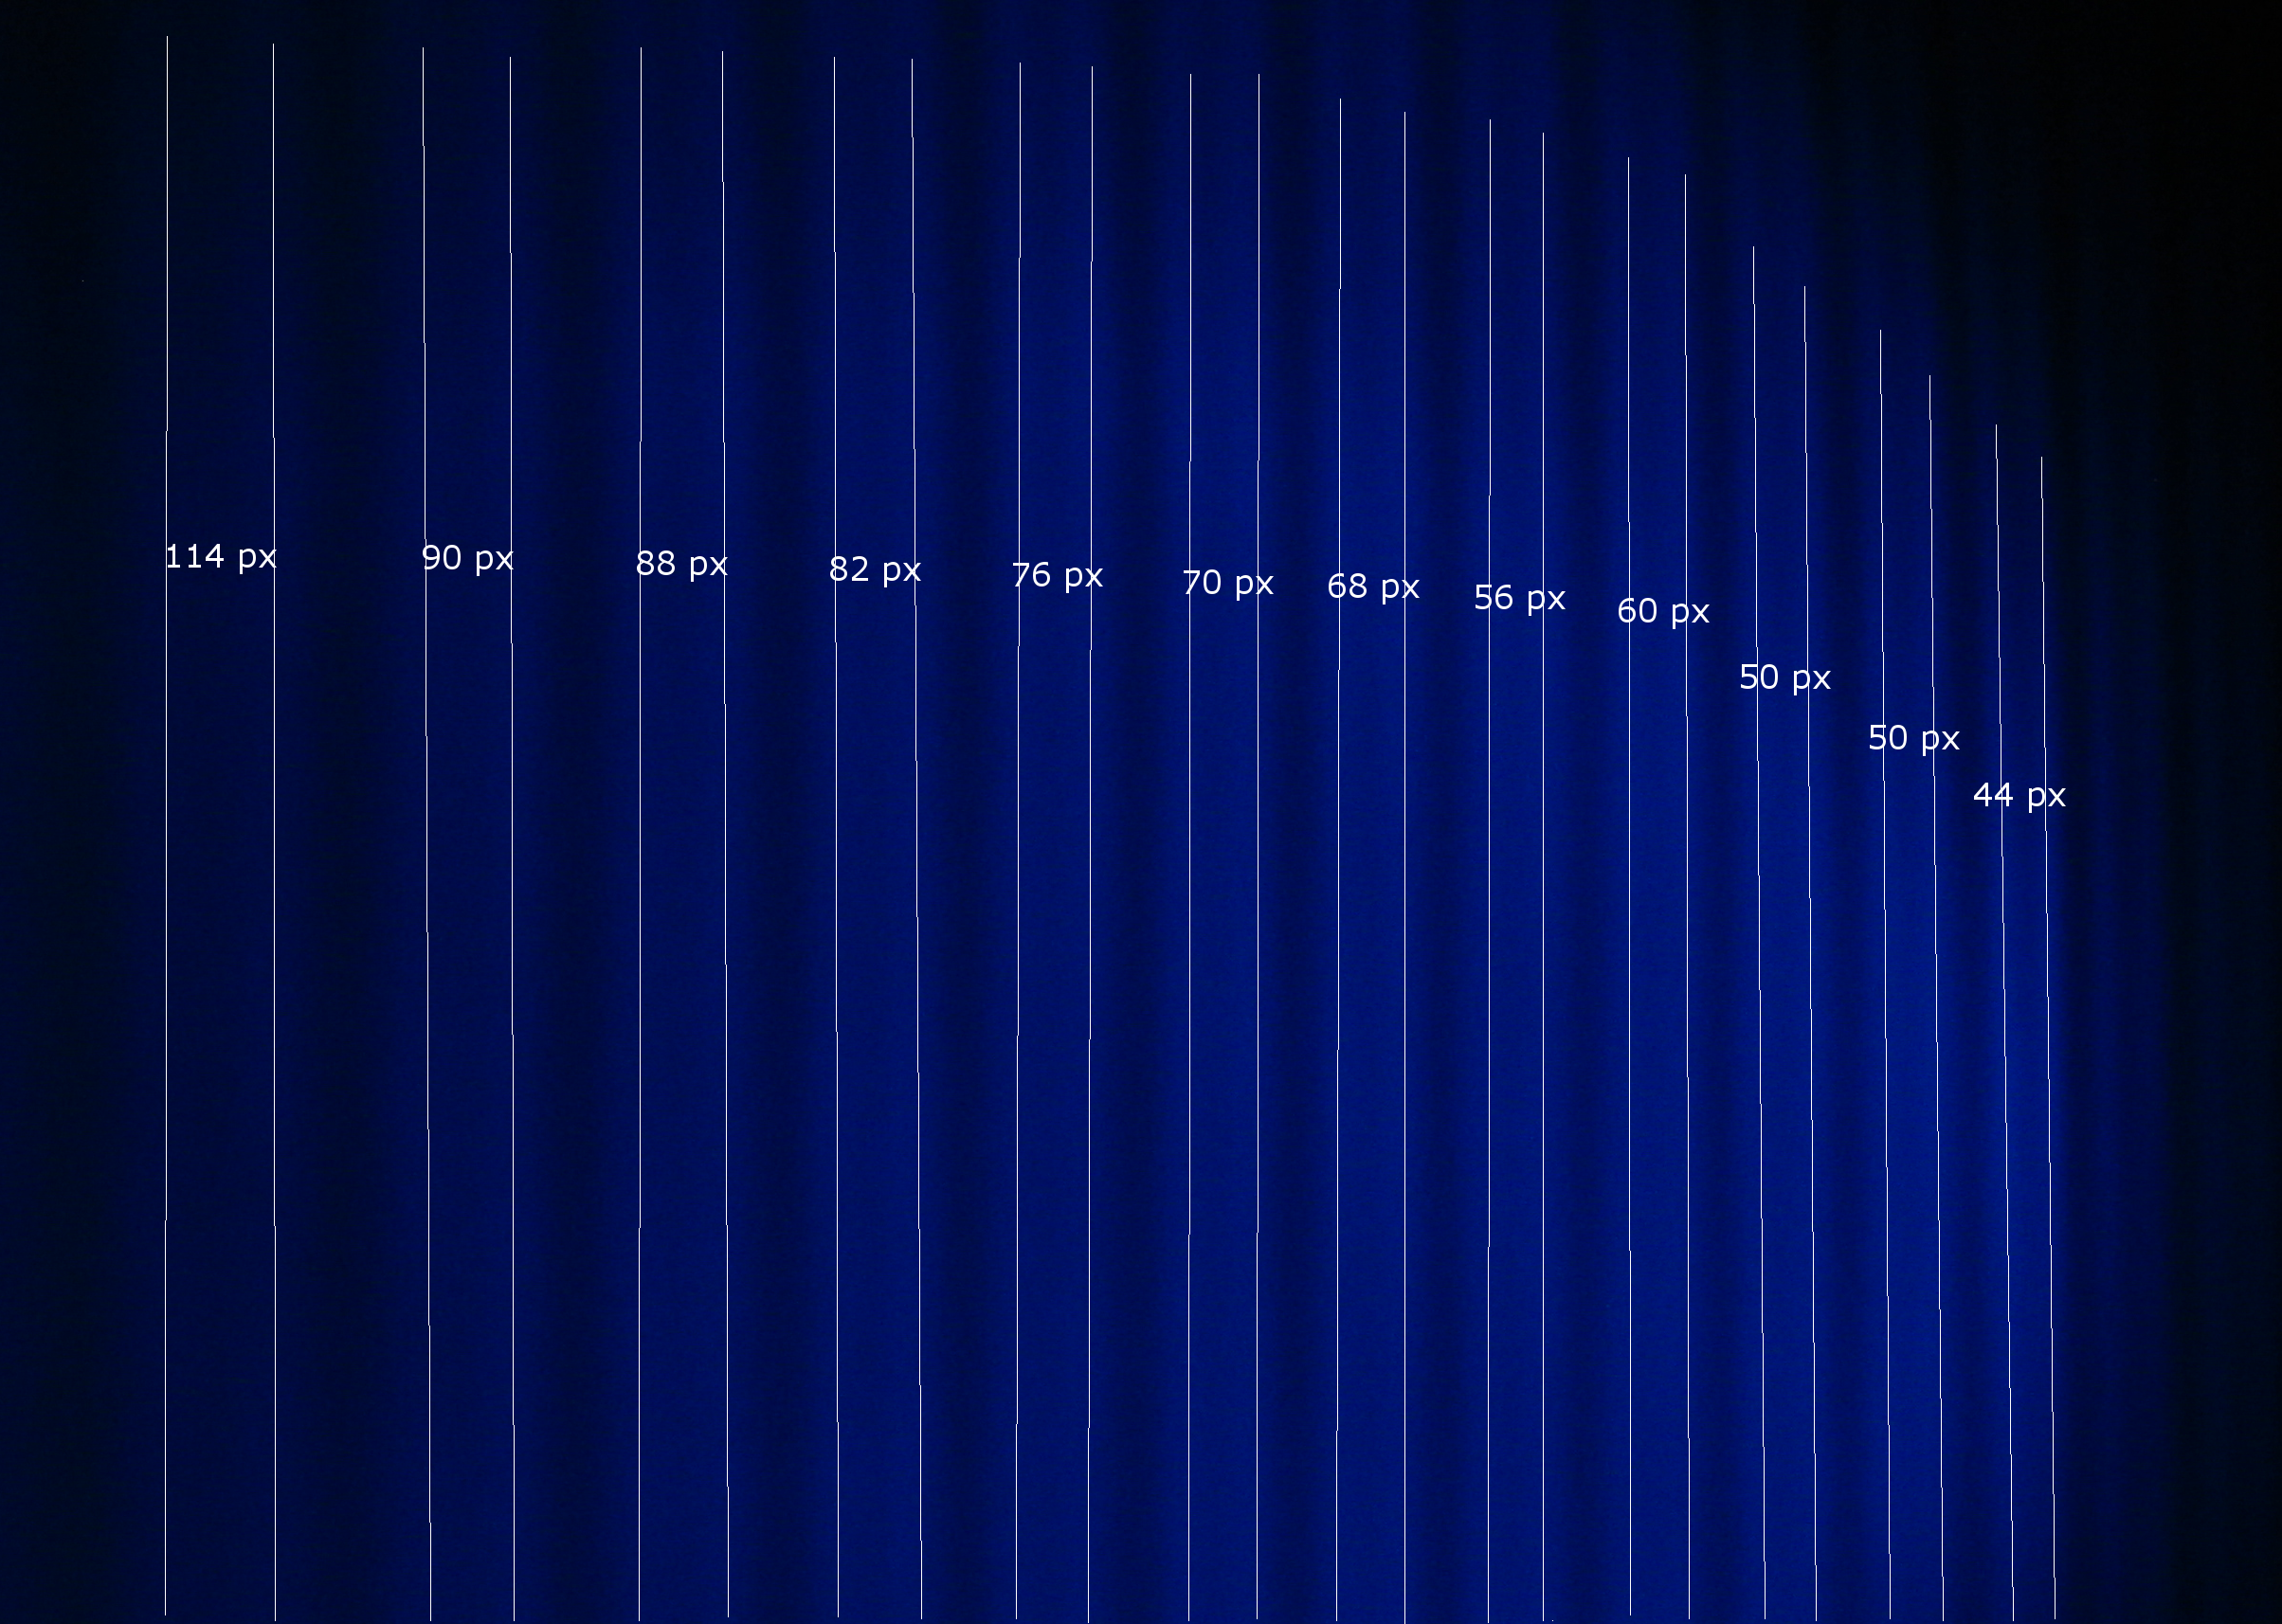
\includegraphics[width=0.95\textwidth]{graphics/auswertung/IMG_1641.png}
  \caption{Blaue $\sigma$-Linie mit Magnetfeld.}
  \label{fig:b_sigma_B}
\end{figure}

\begin{table}
  \centering
  \caption{Messwerte der blauen $\sigma$-Linie.}
  \label{tab:b_sigma}
  \begin{tabular}{S[table-format=3] S[table-format=3] S[table-format=2.3] S[table-format=1.3] @{${}\pm{}$} S[table-format=1.3]}
    \toprule
    {$\upD s \:/\: $px} & {$\symup{\delta} s \:/\: $px} & {$\symup{\delta}\lambda \:/\: $pm} & \multicolumn{2}{c}{Landé-Faktor $g$} \\
    \midrule
    282 & 114 & 5.447 & 1.387 & 0.018 \\
    248 &  90 & 4.890 & 1.245 & 0.016 \\
    208 &  88 & 5.701 & 1.451 & 0.018 \\
    196 &  82 & 5.638 & 1.435 & 0.018 \\
    180 &  76 & 5.689 & 1.448 & 0.018 \\
    162 &  70 & 5.823 & 1.482 & 0.019 \\
    156 &  68 & 5.874 & 1.495 & 0.019 \\
    146 &  56 & 5.168 & 1.316 & 0.017 \\
    140 &  60 & 5.775 & 1.470 & 0.019 \\
    130 &  50 & 5.183 & 1.319 & 0.017 \\
    132 &  50 & 5.104 & 1.299 & 0.017 \\
    110 &  44 & 5.390 & 1.372 & 0.017 \\
    \bottomrule
  \end{tabular}
\end{table}
